\documentclass[journal,12pt,twocolumn]{IEEEtran}

\usepackage{setspace}
\usepackage{gensymb}
\singlespacing
\usepackage[cmex10]{amsmath}

\usepackage{amsthm}

\usepackage{mathrsfs}
\usepackage{txfonts}
\usepackage{stfloats}
\usepackage{bm}
\usepackage{cite}
\usepackage{cases}
\usepackage{subfig}

\usepackage{longtable}
\usepackage{multirow}

\usepackage{enumitem}
\usepackage{mathtools}
\usepackage{steinmetz}
\usepackage{tikz}
\usepackage{circuitikz}
\usepackage{verbatim}
\usepackage{tfrupee}
\usepackage[breaklinks=true]{hyperref}
\usepackage{graphicx}
\usepackage{tkz-euclide}

\usetikzlibrary{calc,math}
\usepackage{listings}
    \usepackage{color}                                            %%
    \usepackage{array}                                            %%
    \usepackage{longtable}                                        %%
    \usepackage{calc}                                             %%
    \usepackage{multirow}                                         %%
    \usepackage{hhline}                                           %%
    \usepackage{ifthen}                                           %%
    \usepackage{lscape}     
\usepackage{multicol}
\usepackage{chngcntr}

\DeclareMathOperator*{\Res}{Res}

\renewcommand\thesection{\arabic{section}}
\renewcommand\thesubsection{\thesection.\arabic{subsection}}
\renewcommand\thesubsubsection{\thesubsection.\arabic{subsubsection}}

\renewcommand\thesectiondis{\arabic{section}}
\renewcommand\thesubsectiondis{\thesectiondis.\arabic{subsection}}
\renewcommand\thesubsubsectiondis{\thesubsectiondis.\arabic{subsubsection}}


\hyphenation{op-tical net-works semi-conduc-tor}
\def\inputGnumericTable{}                                 %%

\lstset{
%language=C,
frame=single, 
breaklines=true,
columns=fullflexible
}
\begin{document}


\newtheorem{theorem}{Theorem}[section]
\newtheorem{problem}{Problem}
\newtheorem{proposition}{Proposition}[section]
\newtheorem{lemma}{Lemma}[section]
\newtheorem{corollary}[theorem]{Corollary}
\newtheorem{example}{Example}[section]
\newtheorem{definition}[problem]{Definition}

\newcommand{\BEQA}{\begin{eqnarray}}
\newcommand{\EEQA}{\end{eqnarray}}
\newcommand{\define}{\stackrel{\triangle}{=}}
\bibliographystyle{IEEEtran}
\raggedbottom
\setlength{\parindent}{0pt}
\providecommand{\mbf}{\mathbf}
\providecommand{\pr}[1]{\ensuremath{\Pr\left(#1\right)}}
\providecommand{\qfunc}[1]{\ensuremath{Q\left(#1\right)}}
\providecommand{\sbrak}[1]{\ensuremath{{}\left[#1\right]}}
\providecommand{\lsbrak}[1]{\ensuremath{{}\left[#1\right.}}
\providecommand{\rsbrak}[1]{\ensuremath{{}\left.#1\right]}}
\providecommand{\brak}[1]{\ensuremath{\left(#1\right)}}
\providecommand{\lbrak}[1]{\ensuremath{\left(#1\right.}}
\providecommand{\rbrak}[1]{\ensuremath{\left.#1\right)}}
\providecommand{\cbrak}[1]{\ensuremath{\left\{#1\right\}}}
\providecommand{\lcbrak}[1]{\ensuremath{\left\{#1\right.}}
\providecommand{\rcbrak}[1]{\ensuremath{\left.#1\right\}}}
\theoremstyle{remark}
\newtheorem{rem}{Remark}
\newcommand{\sgn}{\mathop{\mathrm{sgn}}}
% \providecommand{\abs}[1]{\left\vert#1\right\vert}
% \providecommand{\res}[1]{\Res\displaylimits_{#1}} 
% \providecommand{\norm}[1]{\left\lVert#1\right\rVert}
% %\providecommand{\norm}[1]{\lVert#1\rVert}
% \providecommand{\mtx}[1]{\mathbf{#1}}
% \providecommand{\mean}[1]{E\left[ #1 \right]}
\providecommand{\fourier}{\overset{\mathcal{F}}{ \rightleftharpoons}}
%\providecommand{\hilbert}{\overset{\mathcal{H}}{ \rightleftharpoons}}
\providecommand{\system}{\overset{\mathcal{H}}{ \longleftrightarrow}}
	%\newcommand{\solution}[2]{\textbf{Solution:}{#1}}
\newcommand{\solution}{\noindent \textbf{Solution: }}
\newcommand{\cosec}{\,\text{cosec}\,}
\providecommand{\dec}[2]{\ensuremath{\overset{#1}{\underset{#2}{\gtrless}}}}
\newcommand{\myvec}[1]{\ensuremath{\begin{pmatrix}#1\end{pmatrix}}}
\newcommand{\mydet}[1]{\ensuremath{\begin{vmatrix}#1\end{vmatrix}}}
\numberwithin{equation}{subsection}
\makeatletter
\@addtoreset{figure}{problem}
\makeatother
\let\StandardTheFigure\thefigure
\let\vec\mathbf
\renewcommand{\thefigure}{\theproblem}
\def\putbox#1#2#3{\makebox[0in][l]{\makebox[#1][l]{}\raisebox{\baselineskip}[0in][0in]{\raisebox{#2}[0in][0in]{#3}}}}
     \def\rightbox#1{\makebox[0in][r]{#1}}
     \def\centbox#1{\makebox[0in]{#1}}
     \def\topbox#1{\raisebox{-\baselineskip}[0in][0in]{#1}}
     \def\midbox#1{\raisebox{-0.5\baselineskip}[0in][0in]{#1}}
\vspace{3cm}
\title{Assignment 1}
\author{Buereddy Varuni - EE18BTECH11005}
\maketitle
\newpage
\bigskip
\renewcommand{\thefigure}{\theenumi}
\renewcommand{\thetable}{\theenumi}
Download all latex-tikz codes from 
%
\begin{lstlisting}
https://github.com/varunireddy/-C-DS/blob/main/assignment1/assignment1.tex
\end{lstlisting}
\section{Problem}
Q41. An articulation point in a connected graph is a vertex such that removing the vertex and its incident edges disconnects the graph into two or more connected components.
Let T be a DFS tree obtained by doing DFS in a connected undirected graph G.
Which of the following options is/are correct?
\begin{enumerate}
    \item Root of T can never be an articulation point in G.
    \item Root of T is an articulation point in G if and only if it has 2 or more children.
    \item A leaf of T can be an articulation point in G
    \item If u is an articulation point in G such that x is an ancestor of u in T and y is a descendent of u in T, then all paths from x to y in G must pass through u.
\end{enumerate}
\section{Solution}
Answer : 2, 4
\\
\textbf{Explanation}
\\
Option 2 - Root of T is an articulation point in G if and only if it has 2 or more children. Because, option 2 is an if and only if statement, we have to prove in both the ways. 
\\
\textbf{Case 1:- If root is articulation point then root will have 2 or more children}\\
A vertex is said to be an articulation point if its removal disconnects the graph into 2 or more components. If root is an articulation point. Removal of root node will disconnect the graph. And there is no path between the disconnected components. Therefore, while constructing the DFS tree for graph G, Root vertex is first visited and will have two or more children. 
\\
\textbf{Case 2:- If root vertex has 2 or more children then it is articulation point}\\
Lets say in an undirected graph if root has 2 children then it is true that there is no path between the vertices in left sub-tree and right sub-tree of vertex V (w.r.t DFS traversal tree) because if there had been any path between the left and right sub-tree the in that case if we start with right child then before reaching to the root all the vertices in left sub-tree would have been visited and root had only single child but it is contradiction as root has 2 children and hence there can be no path between the left and right sub-tree of vertex V, thereby making it the ONLY vertex through which vertices in left and right sub-tree are connected.
\\ 
Therefore, Option 2 is correct which also implies Option 1 is wrong.\\
Option 3 - A leaf of T can be an articulation point in G
 This is FALSE because if some vertex is leaf of tree T then all the vertices to which it connects are already been visited which indicates that even without using this leaf vertex there exists path between all of its neighbors and hence it can not be an articulation point.
 \\
 Option 4 - In the figure 1 is the counter example, U is the articulation point in G. And also X is the ancestor of U and Y is the descendent of U. But all the paths from X and Y in G does not pass through U.
\\
Therefore, Option 2 and 4 are correct.\\

\begin{figure}
    \centering
    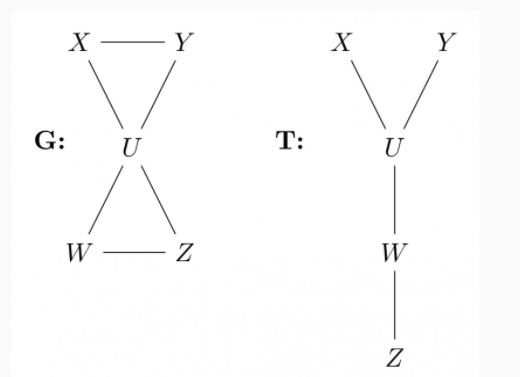
\includegraphics[scale=0.6]{assignment1.png}
    \caption{Figure 1}
    \label{fig: figure1}
\end{figure}
\textbf{Application in Electric circuits:-}\\
\textbf{KIRCHOFFS GRAPH:-}
An electrical circuit can be seen as a connected graph where the nodes of the
electrical circuit are the vertices of the graph and the wires of the electrical cricuit
are the edges of the graph. This will be named Kirchhoff or electrical graph. 
An articulation point in the electric circuit is the node when removed forms two or more different circuits. For example in the figure 2, the node A is the articulation point, which when removed disconnects the circuit.
\begin{figure}
    \centering
    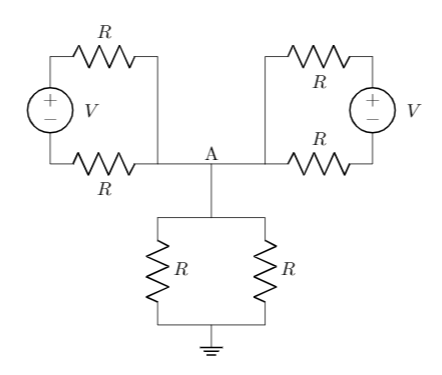
\includegraphics[scale=0.9]{circuit.PNG}
    \caption{Figure 2}
    \label{fig:figure2}
\end{figure}
\end{document}